\section{Knowledge Graph}%
\label{sec:kgraph}
The \ac{hgraph}, discussed in the previous section, spans a lifetime over a single task. In the \ac{hgraph} only the object class is stored for the lifetime of the \ac{hgraph}. When a task is completed, the \ac{hgraph} is deconstructed and learned objects classes are lost. The \ac{kgraph}'s responsibility is to store objects classes for future tasks, and to make an ordering in the edge parameterizations where a edge parameterization comprises of a controller and system model. Estimating which parameterization would be the best candidate is an entire field of research. In this thesis the ordering is made by collecting action feedback on executed action edges and summarizing that feedback in a single metric, the \textit{success factor}. This metric combines two metrics the \acl{PE} and the success-fail ratio of an edge parameterization.\bs

The name \quotes{\acl{kgraph}} originates from the environmental knowledge it contains and its graph structure. Both the \ac{hgraph} and \ac{kgraph} are newly proposed frameworks built from the ground up, with only inspiration from an already existing technique, a backward search. The \ac{kgraph} is in an early stage of development and does therefore not (yet) adhere to any standard that apply to knowledge bases, such as first order-logic~\cite{barwise_introduction_1977,rensink_representing_2004}, relational databases~\cite{atzeni_relational_1993} or more practical, a language such as prologe~\cite{wielemaker_swiprolog_2012}.\bs

\subsection{Definition}
\label{subsec:kgraph_definition}


\todo[inline]{this section}

\subsection{Edge Metrics}
\label{subsec:edge_metrics}
\subsection{Example}
\label{subsec:kgraph_example}



\subsection{Example}%
\label{subsec:kgraph_example}
An example \ac{kgraph} can be visualized in \Cref{fig:kgraph_example}, the parameterization of edges is displayed and the object that the edge controls as image. For clarification, the connected left part with image of the point robot on the center node has 3 outgoing edges that describe robot driving. The connected part on the right with an image of the point robot and the green box on the center node has 2 outgoing edges that describe robot pushing against the green box.\bs

\begin{figure}[H]
    \centering
    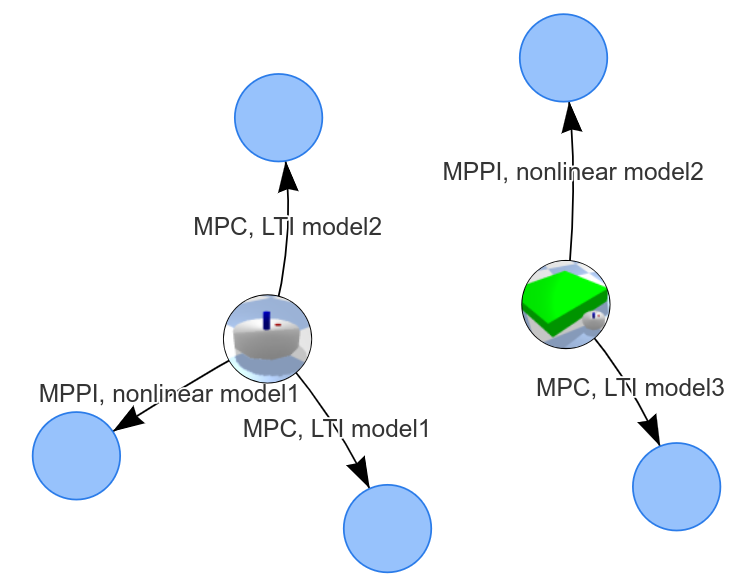
\includegraphics[width=10cm]{figures/kgraph_example}
    \caption{\ac{kgraph} with 3 edges on robot driving, and 2 edges for pushing the green box.}%
    \label{fig:kgraph_example}
\end{figure}

The edges in the figure above display only the edge parameterization, but store more information, mainly the success factor. The blue nodes serve a small purpose, making sure edges can point to a node. The blue nodes could fulfill a larger purpose, that is describing which actuators the edge can control. For example, a mobile robot with robot arm attached can have a set of controllers that only drive the base, a set of controllers that only steer the robot arm and a set that controls both the base and robot arm. In such cases the blue nodes describe which part can of the robot can be actuated. The controllers considered in this thesis control every actuator of the robot, resulting in the blue nodes serving such a small purpose.\bs



now a flowchart is presetend yo
\newpage

\begin{figure}[H] \centering
  \begin{tikzpicture}[node distance = 4.5cm, line width=1pt]
    % Nodes
    \node [block, fill=green!50] (first) {Update existing edge with new feedback};
    
    % legend 
    \node[text width=2.8cm, yshift=1cm, right of=first, text centered, rounded corners, minimum height=1em, label={[name=lab, yshift=0.4cm, left]\textbf{Legend}}, node distance=7cm] (legend1) {\small Update KGraph};
    \node[rectangle, draw, left of=legend1, fill=green!50, rounded corners, minimum height=1em, minimum width=1cm, node distance=2cm] (legend1color) {};
    \node[text width=2.8cm, below of=legend1, text centered, minimum height=1em, node distance=0.7cm] (legend2) {\small Query KGraph};
    \node[rectangle, draw, left of=legend2, fill=red!40, rounded corners, minimum height=1em, minimum width=1cm, node distance=2cm] (legend2color) {};
   
    
    % nodes, first row 
    \node [decision, below of=first, node distance=4.5cm, fill=red!40, text width=7.0em] (has_controller) {Does this parameterization exist in one of the center node's outgiong edges?};
    \node [block, left of=has_controller, fill=green!50] (new_transition) {Generate new edge with feedback edge with feedback existing node};
    
    % nodes, second row 
    \node [decision, fill=red!40, below of=has_controller, node distance=6cm, text width=6.0em] (obj_exist) {Does this object exist in a center node in the \ac{kgraph}?};

  \node [decision, fill=red!40, right of=obj_exist, node distance=4.5cm, text width=6.0em] (obj_exist2) {Does this object exist in a center node in the \ac{kgraph}?};
    \node [block, yshift=-3cm, above= of obj_exist2, node distance=-1.8cm] (send_feedback) {Send ordered list with controllers and models};
    
    \node [block, fill=green!50, left of=obj_exist] (new_object) {Generate new center node, side node and an edge with feedback};
    \node [block, right of=obj_exist2, node distance=3.8cm] (no_obj) {send empty list};
   
    % Edges
    \draw[stealth-] (obj_exist) -- node[left, at end]{action feedback} +(0,-3.5cm);
    \draw[-stealth] (obj_exist.west) -- node[above]{no} (new_object.east);
    \draw[-stealth] (obj_exist.north) -- node[left]{yes} (has_controller.south);
    \draw[-stealth] (has_controller.north) -- node[left]{yes} (first.south);
    \draw[-stealth] (has_controller.west) -- node[above]{no} (new_transition.east);
    
    \draw[-stealth] (obj_exist2.east) -- node[above]{no} (no_obj.west);
    \draw[-] (no_obj.east) -- +(0.7cm, 0);
    \draw[stealth-] (obj_exist2) -- node[left, at end]{action suggestion?} +(0,-3.5cm);
    \draw[-stealth] (obj_exist2.north) -- node[left]{yes} (send_feedback.south);
    \draw[-stealth] (send_feedback.east) -| node[at end, left]{action suggestion} +(4.5cm, -8.4cm);
\end{tikzpicture}
\caption{Flowchart displaying the knowledge graph's workflow.}%
\label{figure: flowchart_kgraph} 
\end{figure}


The \ac{kgraph} fulfills two goals. It stores information on whether an object can be manipulated and stores edge parameterizations from the highest success factor to the lowest success factor per object. Information if objects can be manipulated to prevent the \ac{halgorithm} from trying to push unmovable objects.\bs

% \subsection{Edge Metrics}%
% \label{subsec:edge_metrics}
% \todo{Corrado: rephrase good and bad to sound like a professional cunt}
% The \ac{kgraph} keeps an ordered list of `good' and `bad' edge arguments (controller and system model). `Good' and `bad' are defined by edge metrics; these metrics are created after the completion of an edge, regardless of whether the edge was completed or failed. An indication is given on why specific metrics matter in \Cref{table:review_edge_metrics}.

% \noindent
% \begin{table}[H]
% \centering
% \begin{tabular}%
% {>{\raggedright\arraybackslash}p{0.25\textwidth}%
% >{\raggedright\arraybackslash}p{0.65\textwidth}}
% \acf{PE}&  To better compare prediction errors the \ac{PE} is summarized and average \ac{PE}. The average \ac{PE} indicates an accurate system model but can give misleading results since \ac{PE} is also an indicator of unexpected collisions. Prediction error should thus only be used if there are no collisions detected. The average \ac{PE} has more flaws since outliers mostly determine the average. For the largest part, some unfortunate outliers in the \ac{PE} might determine the average \ac{PE}. The average \ac{PE} will thus not be used because it is not robust enough.\\
% % \acf{TE}& For a low \ac{TE}, the system model must be close to the real motion equations to yield a feasible path, the controller must be well tuned to be able to track that path and the controller and system model must be in collaboration, because the controller uses the system model to calculate system input. A low \ac{TE} tells multiple things, whilst a high \ac{TE} would indicate improvements could be gained in the controller, the system model or their collaboration.\\
% ratio num\_succesfully completed edges and num\_total edges & Over time, the \ac{kgraph} can recommend the same edge arguments multiple times. Logging the ratio of succeeding edges vs total edges builds an evident portfolio. Still, this metric has to be taken with a grain of salt because edges with equal edge arguments perform similar actions e.g.~pushing an object through a wide corridor is compared to pushing the same object through a narrow corridor. One could say \quotes{comparing apples with pears}\todo{Corrado: But then you would have task-specific metrics right? Meaning a knowledge graph for when you do pushes in open space and one for small corridors? I don’t know if this would scale. To make sense of the metric this metric should be task specific though }.\\
% the final position and \newline displacement error & The quality of the result is measured in the final position and displacement error. The importance should thus be stressed when ordering edge arguments.\\
% planning time& With system identification, path estimation, motion or manipulation planning, the planning time can vary in orders of magnitude between simple or more complex approaches.\\
% run time& Also known as execution time, would be a quality indicator if start- and target states were equal. Edges are recommended to solve similar tasks where the path length between the start and target state differs. Thus planning time is not of any use to rank edges.\\
% completion time = \newline run time + planning time & With the same argumentation as run time, completion time is not used to rank edges.\\
% \end{tabular}
% \caption{The edge metrics employed to establish a ranking of edge parameterizations.}
% \label{table:review_edge_metrics}
% \end{table}

% \todo{Corrado: So why do we have all these metrics if you do not consider them? Shouldn’t you normalize the metrics such that they are at least comparable with each other in similar yet differe tasks?}
